77. \begin{figure}[ht!]
\center{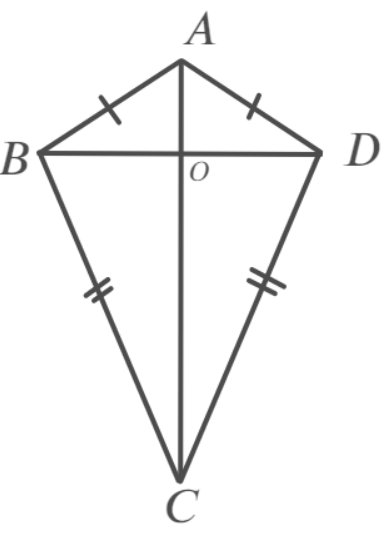
\includegraphics[scale=0.35]{g77.png}}
\end{figure}\\
$\left.\begin{array}{l}AB=AD,\\
BC=CD,\\
AC\text{--- общая.}  \end{array}
ight\}\Rightarrow \Delta ABC=\Delta ADC\text{ по III признаку.}$ Значит, $\angle BAC=\angle DAC$ и $AO$ является биссектрисой равнобедренного треугольника $ABD,$ а значит является и высотой, ч.т.д.\\
